\documentclass{article}

\usepackage[hangul]{kotex}
\usepackage[a4paper, margin=1in]{geometry}

\usepackage{hyperref}

\usepackage{graphicx}
\usepackage{float}

\usepackage{tcolorbox}
\tcbuselibrary{listings}

\usepackage{tikz}

\newcommand\code[1]{
  \texttt{\large{#1}}
}


\title{데이터베이스시스템 프로젝트 1}
\author{이주헌 (20191629)}
\date{2024년 4월 19일}

\begin{document}
\pagenumbering{gobble}
\maketitle
\newpage

\pagenumbering{arabic}
\section{개요}

본 프로젝트에서는 에서 제공하는 서비스를 참고하여, 서울 지역의 부동산 목록을 저장, 관리할 수 있는 데이터베이스를 설계한다.
설계한 데이터베이스는 ER Diagram, Relational Schema Diagram으로 표현하였고, 이 데이터베이스 내용을 조회하는 SQL 쿼리 예제 몇 가지도 함께 제시한다.

\section{데이터베이스 요구사항}

주어진 샘플 쿼리와 직방 웹사이트로부터 아래 요구사항 목록을 추려낼 수 있다.

\begin{itemize}
\item 시 \cdot 군 \cdot 구 기준으로 매물을 정렬할 수 있다.
\item 각 매물의 전경이나 내부 사진을 보여 줄 수 있다.
\item 건물 소유주가 직접 거래하거나 부동산 중개업자를 통해 거래할 수 있다.
\item 거래가 발생하면, 언제 거래가 발생했는지 함께 기록한다.
\end{itemize}

\section{ER 다이어그램}

아래는 직방에 올라온 부동산 매물을 나타내는 ER 다이어그램이다.

각 엔티티은 이름 뒤에 \code{\_id}를 붙인 이름으로 된 기본 키를 가지고 있으며, 해당 키의 타입은 UUID이다.
따로 UUID 타입이 없는 데이터베이스에서는 \code{VARCHAR(36)} 타입으로 대체할 수 있다.

\begin{figure}[H]
  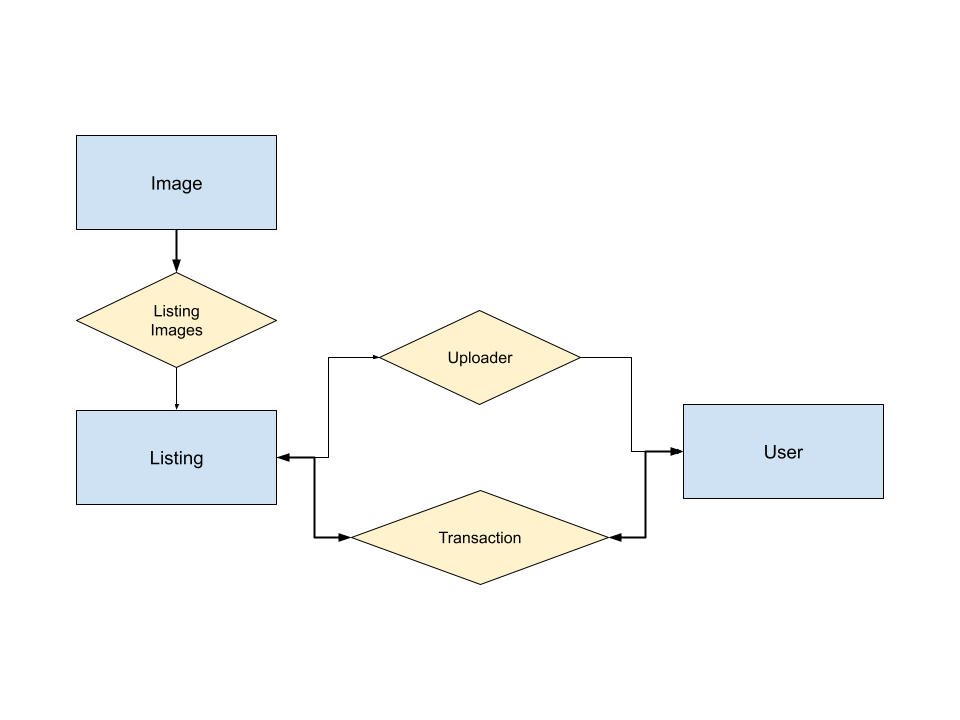
\includegraphics[width=\linewidth]{er-diagram.png}
  \caption{직방 데이터베이스를 나타내는 ER 다이어그램.}
  \label{fig:er-diagram}
\end{figure}

\begin{figure}[H]
  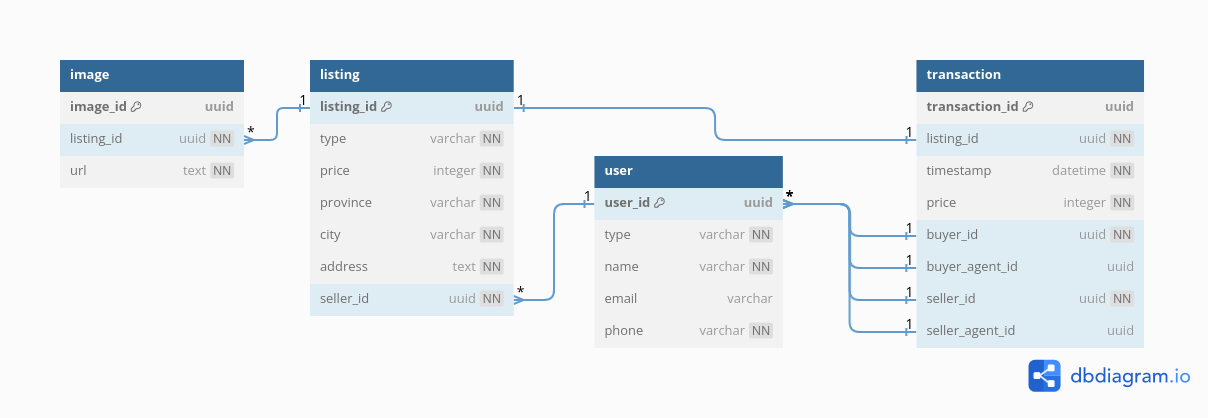
\includegraphics[width=\linewidth]{schema-diagram.png}
  \caption{직방 데이터베이스 스키마를 나타내는 다이어그램.}
  \label{fig:schema-diagram}
\end{figure}
\newpage

\subsection{매물 정보 엔티티}

\code{listing} 엔티티는 직방에 올라온 모든 매물을 나타낸다.
모든 속성은 NULL일 수 없다.

\begin{itemize}
\item \textbf{type}: 매물의 종류를 나타내는 문자열이다. ``apartment'', ``villa'', ``oneroom'', ``officetel'', ``detached'' 중 하나여야 한다.
\item \textbf{timestamp}: 매물이 등록된 날짜이다.
\item \textbf{price}: 매물의 가격으로, 정수이다.
\item \textbf{province}: 매물이 위치한 광역자치단체 이름이다.
\item \textbf{city}: 매물이 위치한 시 \cdot 군 \cdot 구 이름이다.
\item \textbf{address}: 매물의 주소이다. 항상 도로명주소로 저장해야 한다.
\item \textbf{bedroom\_count}: 매물의 침실 개수이다.
\item \textbf{bathroom\_count}: 매물의 화장실 개수이다.
\item \textbf{seller\_id}: 매물을 등록한 사용자의 ID이다. \code{user} 엔티티를 가리키는 외래 키(foreign key)이다.
\end{itemize}

\subsection{매물 사진 엔티티}

\code{image} 엔티티는 각 매물에 등록된 사진을 저장한다.
모든 속성은 NULL일 수 없다.

\begin{itemize}
\item \textbf{listing\_id}: 해당 사진이 등록된 매물의 ID이다. \code{listing} 엔티티를 가리키는 외래 키이다.
\item \textbf{url}: 실제 사진이 저장된 URL이다.
\end{itemize}

\subsection{직방 사용자 엔티티}

\code{user} 엔티티는 직방 회원을 나타낸다.
\textbf{email}을 제외한 다른 속성은 NULL일 수 없다.

\begin{itemize}
\item \textbf{name}: 회원의 이름이다.
\item \textbf{type}: 회원의 종류이다. 일반 회원은 ``regular'', 부동산 중개업자 회원은 ``agent''이다.
\item \textbf{email}: 회원의 이메일 주소이다. 아래 전화번호로 연락할 수 있으므로 이메일은 NULL일 수 있다.
\item \textbf{phone}: 회원의 전화번호이다.
\end{itemize}

\subsection{매매 계약 엔티티}

\code{transaction} 엔티티는 성사된 매매 계약을 나타낸다.
중개업자를 경유해서 맺은 계약이 아닐 수도 있으니 \textbf{*\_agent\_id} 속성은  NULL일 수 있다.

\begin{itemize}
\item \textbf{listing\_id}: 거래한 매물의 ID이다. \code{listing} 엔티티를 가리키는 외래 키이다.
\item \textbf{timestamp}: 계약이 성사된 날짜와 시간이다.
\item \textbf{price}: 실제 매매 가격이다.
\item \textbf{\{buyer,seller\}\_[agent\_]id}: 각각 구매자, 판매자의 ID이며, 중개업자는 \textbf{agent}가 포함된 속성에 저장된다. 모두 \code{user} 엔티티를 가리키는 외래 키이다.
\end{itemize}

\subsection{매물 이미지 관계}

하나의 매물 등록 게시글은 여러 개의 사진을 가질 수 있다.
따라서, \code{listing} 엔티티와 \code{image} 엔티티는 \textbf{일대다(1:n)} 관계를 맺고 있다.

\subsection{등록한 사용자 관계}

직방에 등록된 모든 매물의 소유주는 한 명이다.
해당 매물이 공동명의로 되어 있더라도, 등록자는 한 명으로 간주한다.
따라서, \code{listing} 엔티티와 \code{user} 엔티티는 소유주에 대하여 약한(weak) \textbf{일대일(1:1)} 관계를 맺고 있다.

\subsection{계약 관계}

매물과 사용자가 맺을 수 있는 관계 중에서 계약 관계는 조금 복잡하다.
하나의 매물에 대하여 여러 사용자가 계약에 참여할 수 있고, 각 사용자는 여러 매물을 사고팔 수 있다.
따라서, \code{listing} 엔티티와 \code{user} 엔티티는 계약 관계에 대하여 \textbf{다대다(n:n)} 관계를 맺고 있다.
이 관계는 위에서 보인 \code{transaction} 엔티티가 추상화한다.

\section{쿼리 예제}

아래는 위에서 정의한 스키마를 이용하여 문제를 해결하는 SQL 쿼리 예제이다.

\subsection{마포구의 10억원대 매물 찾기}

아래 SQL문은 마포구에 있는 10억원대 매물을 찾는 쿼리이다.

\begin{tcblisting}{
    listing only,
    listing options = {
      basicstyle = \ttfamily,
      keywordstyle = \color{blue},
      language = sql,
      columns = fullflexible
    },
    title = SQL 쿼리
  }
  SELECT address
  FROM listing
  WHERE
    province = 'Seoul'
    AND city = 'Mapo-gu'
    AND (1000000000 < price AND price < 1500000000);
\end{tcblisting}
\newpage

\subsection{8학군에서 침실 4개 이상, 화장실 2개인 방 찾기}

아래 SQL문은 8학군(강남구, 서초구)에서 침실 4개 이상이 있고, 화장실이 2개인 매물을 찾는 쿼리이다.

\begin{tcblisting}{
    listing only,
    listing options = {
      basicstyle = \ttfamily,
      keywordstyle = \color{blue},
      language = sql,
      columns = fullflexible
    },
    title = SQL 쿼리
  }
  SELECT address
  FROM listing
  WHERE
    province = 'Seoul'
    AND (city = 'Gangnam-gu' OR city = 'Seocho-gu')
    AND bathroom_count = 2
    AND bedroom_count >= 4;
\end{tcblisting}
\newpage

\subsection{2022년 최고의 부동산 중개업자 찾기}

아래 SQL문은 2022년 가장 많은 수익을 올린 부동산 중개업자를 찾는 쿼리이다.

\begin{tcblisting}{
    listing only,
    listing options = {
      basicstyle = \ttfamily,
      keywordstyle = \color{blue},
      language = sql,
      columns = fullflexible
    },
    title = SQL 쿼리
  }
  SELECT
    u.name AS agent_name
    SUM(t.price) AS total_sales
  FROM
    transaction t
  JOIN
    user u ON seller_agent_id = u.user_id
  WHERE
    u.type == 'agent'
    AND DATE(t.timestamp) >= '2022-01-01'
    AND DATE(t.timestamp) >= '2022-12-31'
  GROUP BY
    u.name
  ORDER BY
    total_sales DESC
  LIMIT 1;
\end{tcblisting}
\newpage

\subsection{부동산 중개업자의 성과 보기}

아래 SQL문은 각 부동산 중개업자의 평균 성과를 구한다.

\begin{tcblisting}{
    listing only,
    listing options = {
      basicstyle = \ttfamily,
      keywordstyle = \color{blue},
      language = sql,
      columns = fullflexible
    },
    title = SQL 쿼리
  }
  SELECT
    u.name AS agent_name,
    AVG(t.price) AS average_selling_price,
    AVG(EXTRACT(EPOCH FROM (t.timestamp - l.timestamp))
      / (60 * 60 * 24)) AS average_time_on_market_days
  FROM
    transaction t
  JOIN
    listing l ON t.listing_id = l.listing_id
  JOIN
    user u ON t.seller_agent_id = u.user_id
  WHERE
    u.type = 'agent'
    AND DATE(t.timestamp) >= '2022-01-01'
    AND DATE(t.timestamp) <= '2022-12-31'
  GROUP BY
    u.name;
\end{tcblisting}
\newpage

\subsection{가장 비싼 매물 사진 찾기}

아래 SQL문은 집 종류별로 가장 비싼 집을 찾아 그 집의 사진을 보여준다.

\begin{tcblisting}{
    listing only,
    listing options = {
      basicstyle = \ttfamily,
      keywordstyle = \color{blue},
      language = sql,
      columns = fullflexible
    },
    title = SQL 쿼리
  }
  WITH most_expensive_listings AS (
    SELECT
      l.type,
      l.listing_id,
      MAX(l.price) AS max_price
    FROM
      listing l
    WHERE
      l.type IN ('apartment', 'villa', 'oneroom', 'detached')
    GROUP BY
      l.type
  ),
  most_expensive_listings_ids AS (
    SELECT
      l.listing_id
    FROM
      listing l
    JOIN
      most_expensive_listings m ON l.type = m.type
      AND l.price = m.max_price
  )
  SELECT
    i.url AS image_url,
    l.listing_id,
    l.type
  FROM
    image i
  JOIN
    listing l ON i.listing_id = l.listing_id
  JOIN
    most_expensive_listings_ids m
      ON l.listing_id = m.listing_id;
\end{tcblisting}
\newpage

\subsection{구매 계약하기}

아래 SQL문은 \textbf{홍길동}이라는 사람이 \textbf{김영희} 공인중개사를 통해 위에서 구한 가장 비싼 집을 정가에 구매하는 상황을 만든다.

\begin{tcblisting}{
    listing only,
    listing options = {
      basicstyle = \ttfamily,
      keywordstyle = \color{blue},
      language = sql,
      columns = fullflexible
    },
    title = SQL 쿼리
  }
  INSERT INTO transaction (
    transaction_id,
    listing_id,
    timestamp,
    price,
    buyer_id,
    buyer_agent_id,
    seller_id,
    seller_agent_id
  )
  VALUES (
    '1842f3aa-c9fa-4407-addb-542984c3e040',
    (SELECT listing_id FROM most_expensive_listings LIMIT 1),
    NOW(),
    (SELECT max_price FROM most_expensive_apartment LIMIT 1),
    (SELECT user_id FROM user WHERE name = '홍길동'),
    (SELECT user_id FROM user WHERE name = '김영희' AND type = 'agent'),
    (
      SELECT seller_id
      FROM listing
      WHERE listing_id = (SELECT listing_id FROM most_expensive_apartment)
    ),
    (
      SELECT seller_agent_id
      FROM listing
      WHERE listing_id = (SELECT listing_id FROM most_expensive_apartment)
    )
  );

  UPDATE listing
  SET status = 'sold'
  WHERE listing_id = (SELECT listing_id FROM most_expensive_apartment);
\end{tcblisting}
\newpage

\subsection{새 공인중개사 등록하기}

아래 SQL문은 새 공인중개사 \textbf{김철수}를 등록한다.

\begin{tcblisting}{
    listing only,
    listing options = {
      basicstyle = \ttfamily,
      keywordstyle = \color{blue},
      language = sql,
      columns = fullflexible
    },
    title = SQL 쿼리
  }
  INSERT INTO user (user_id, type, name, phone)
  VALUES (
    '620ebcc8-95e9-4593-9881-1f0aa44ee460',
    'agent',
    '김철수',
    '010-1234-5678'
  );
\end{tcblisting}

\end{document}
